\documentclass[letterpaper,10pt]{article}

\usepackage{titling}
\usepackage{listings}
\usepackage{url}
\usepackage{setspace}
\usepackage{subfig}
\usepackage{sectsty}
\usepackage{pdfpages}
\usepackage{colortbl}
\usepackage{multirow}
\usepackage{multicol}
\usepackage{relsize}
\usepackage{amsmath}
\usepackage{wasysym}
\usepackage{fancyvrb}
\usepackage{amssymb}
\usepackage{ifsym}
\usepackage{amsmath,amssymb,amsthm,graphicx,xspace}
\usepackage[titlenotnumbered,noend,noline]{algorithm2e}
\usepackage[compact]{titlesec}
\usepackage{XCharter}
\usepackage[T1]{fontenc}
\usepackage{tikz}
\usetikzlibrary{arrows,automata,shapes,trees,matrix,chains,scopes,positioning,calc}
\tikzstyle{block} = [rectangle, draw, fill=blue!20, 
    text width=2.5em, text centered, rounded corners, minimum height=2em]
\tikzstyle{bw} = [rectangle, draw, fill=blue!20, 
    text width=4em, text centered, rounded corners, minimum height=2em]

\definecolor{namerow}{cmyk}{.40,.40,.40,.40}
\definecolor{namecol}{cmyk}{.40,.40,.40,.40}

\let\LaTeXtitle\title
\renewcommand{\title}[1]{\LaTeXtitle{\textsf{#1}}}


\newcommand{\handout}[5]{
  \noindent
  \begin{center}
  \framebox{
    \vbox{
      \hbox to 5.78in { {\bf ECE356: Database Systems } \hfill #2 }
      \vspace{4mm}
      \hbox to 5.78in { {\Large \hfill #4  \hfill} }
      \vspace{2mm}
      \hbox to 5.78in { {\em #3 \hfill} }
    }
  }
  \end{center}
  \vspace*{4mm}
}

\newcommand{\lecture}[3]{\handout{#1}{#2}{#3}{Lecture #1}}
\newcommand{\tuple}[1]{\ensuremath{\left\langle #1 \right\rangle}\xspace}

\addtolength{\oddsidemargin}{-1.000in}
\addtolength{\evensidemargin}{-0.500in}
\addtolength{\textwidth}{2.0in}
\addtolength{\topmargin}{-1.000in}
\addtolength{\textheight}{1.75in}
\addtolength{\parskip}{\baselineskip}
\setlength{\parindent}{0in}
\renewcommand{\baselinestretch}{1.5}
\newcommand{\term}{Winter 2018}

\singlespace


\begin{document}

\lecture{ 8 ---  Modelling Diagrams }{\term}{Jeff Zarnett}

\section*{Modelling Diagrams}

We have talked at some length about the tools for defining the database, but we really should spend significant time on good design. Knowing how hammers work is not enough; we also need to understand what good architectural plans look like.

The first thing we would like to watch out for is redundancy in the database and eliminate it wherever possible. In short, if there is redundant data then there is the potential for data to get out of date or be in some other inconsistent state. 

When we have some data that we would like to represent we need to turn it into some database tables. Going directly from some ideas about what data we need to the tables is sometimes difficult and may produce undesirable results. Instead, we should devise a plan for how it should be implemented and for that we will create diagrams. Diagrams are done on paper or a whiteboard or similar and it is very easy to visualize, understand, and change the design at that stage.

We are going to use Entity-Relationship diagrams (E-R diagrams) as our method for modelling the entities in the database as well as their relations. Entity-relationship diagrams have the following symbols and their meanings~\cite{dsc}:

\begin{itemize}
	\item \textbf{Divided Rectangles} represent an entity; an entity has a title (the top part) and a list of the attributes of that entity (the bottom part).
	\item \textbf{Diamonds} represent a relationship set.
	\item \textbf{Undivided Rectangles} represent the attributes of a relationship set. 
	\item \textbf{Lines} link entity sets to relationship sets.
	\item \textbf{Dashed Lines} linked the attributes of a relationship set to its relationship set.
	\item \textbf{Double lines} indicate total participation of an entity in a relationship set.
	\item \textbf{Double Diamonds} represent identifying relationship sets linked to weak entity sets.
\end{itemize}

We'll come back to those last two items later. Note also that in rectangles, attributes that are or form part of the primary key are underlined. Consider an example below:

\begin{center}
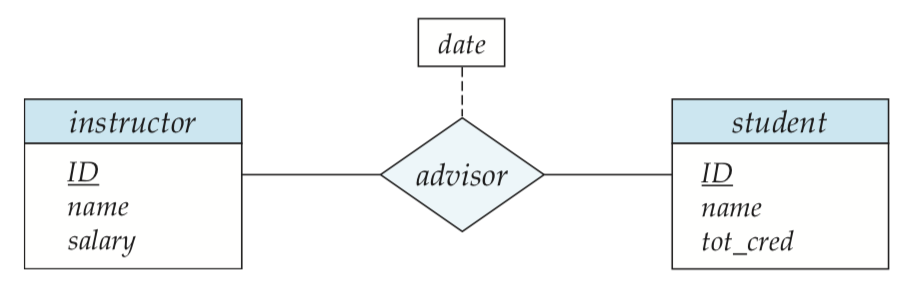
\includegraphics[width=0.55\textwidth]{images/er-with-attr}\\
E-R diagram showing relationship between instructors and students, with attributes~\cite{dsc}.
\end{center}

In this case we have a relationship between instructor and student called ``advisor'' and that relationship has an associated date. What sort of relationship is shown here? This is a many-to-many relationship. To decide as to whether that makes sense, let's think about real life: a professor can advise multiple graduate students, and a graduate student can have more than one advisor (for example, two of them). The diagrams below show the other possibilities:

\begin{center}
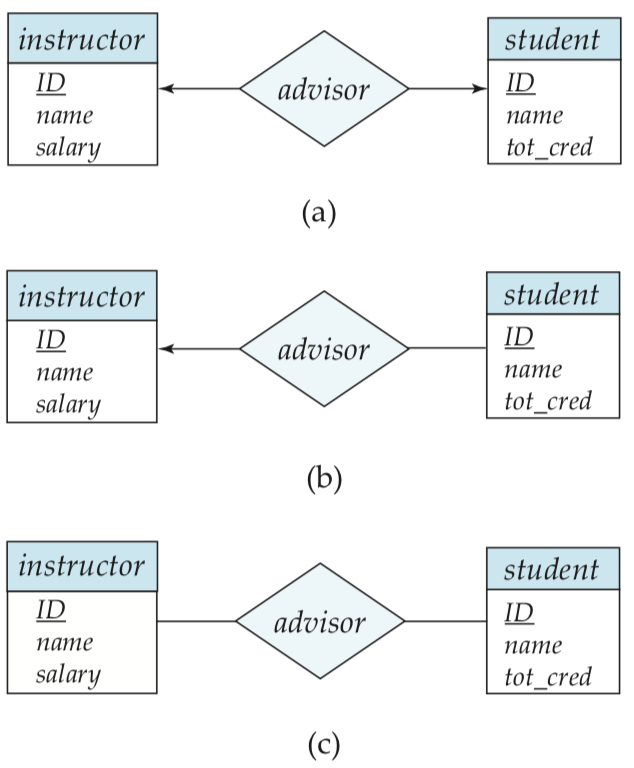
\includegraphics[width=0.35\textwidth]{images/advisor-relationship}\\
E-R diagram with (a) one-to-one, (b) one-to-many, and (c) many-to-many relationships~\cite{dsc}.
\end{center}

If we want to show some more specific rules that allow us to be more specific than just one vs. many, we can apply some numbers to the lines. In the diagram below, an instructor can have zero or more students and a student can have exactly one advisor.

\begin{center}
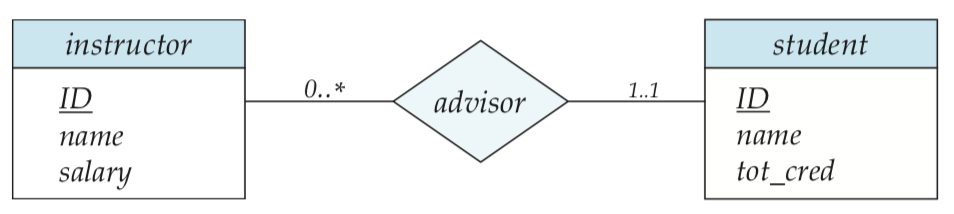
\includegraphics[width=0.55\textwidth]{images/cardinality-limits}\\
E-R diagram showing cardinality limits~\cite{dsc}.
\end{center}

There is no reason why a relationship must be binary. A table may reference itself, as in the case of courses that have prerequisites. If that is so, then assigning names to the relations help to differentiate. Or a relation may involve many relations as in a ternary relationship:

\begin{center}
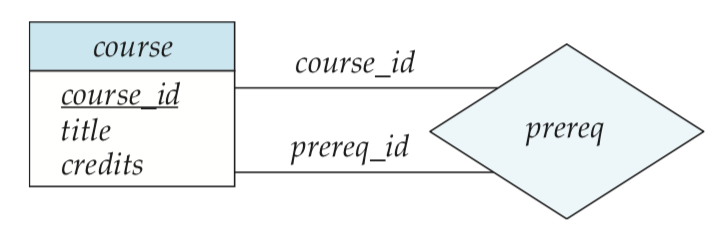
\includegraphics[width=0.45\textwidth]{images/prereq}
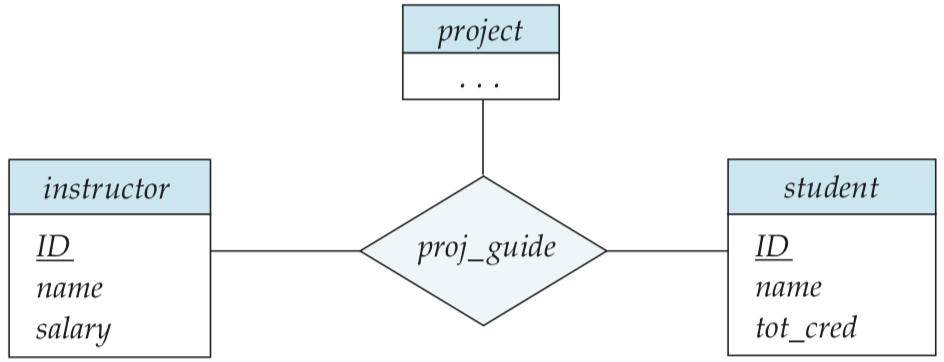
\includegraphics[width=0.45\textwidth]{images/er-ternary}\\
Non-binary E-R diagrams; unary and ternary respectively~\cite{dsc}.
\end{center}

\paragraph{Weak Entity Sets.} Weak entity sets are not entities that do not even lift. Instead, they are entities that are dependent on another entity, namely, one that cannot be identified uniquely based on its own attributes. The example that builds on this ``university'' model is a section: a section of a course, such as 001, is dependent on a course in a particular term. 

Suppose that a course has an id, name, and code. A section has a section number, year, and term. A particular course, ECE 356, will have one or more sections, e.g. 001. But the attributes of the section on their own (001, 2018, Winter) are not enough to uniquely identify a single course. Because at least one another course, such as ECE 459, also has a section that matches (001, 2018, Winter). To differentiate between two sections that match on those same criteria we need a course number, but the course number isn't a part of the section entity. That is part of the course entity. And this is what makes the section entity a weak entity.

More formally, an entity that on its own does not possess sufficient attributes to form a primary key is a weak entity; one that is not weak is a strong entity. A weak entity set is associated with another entity, called its identifying set or its owner entity set~\cite{dsc}.

In a practical sense the weak entity will probably have some attribute added to it that identifies which strong entity the weak entity belongs to. That is called the \textit{discriminator}. That would mean some attribute added to the section entity that references a particular course. Still, that is an implementation detail that plays no role in the E-R diagram, which looks like the diagram below:

\begin{center}
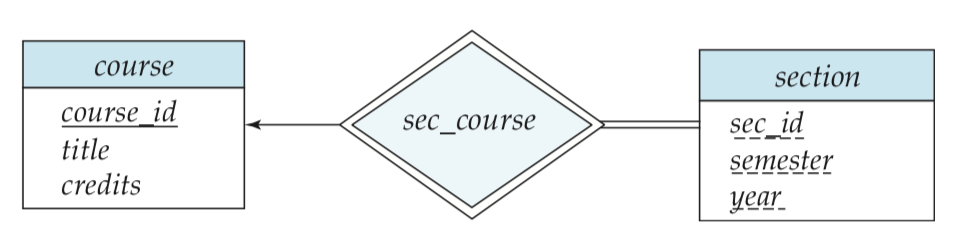
\includegraphics[width=0.55\textwidth]{images/weak-entity-set}\\
E-R diagram with weak entity set~\cite{dsc}.
\end{center}

It is worth noting that the weak entity shown in the diagram has some slight differences versus a strong entity. The attributes are underlined with a dashed line and the relationship is modelled with a double diamond. It also uses double lines between section and sec\_course that indicates total participation: every section MUST be associated with a single course.

We could choose a different option, of course, and add some sort of unique identifier to the section that would promote the weak entity to a strong one. But that doesn't necessarily make logical sense in the context of the application; a section doesn't make sense on its own and giving it a unique identifier does not really correspond with reality: a section is logically dependent on the course, isn't it?

Weak entity sets can exist in other configurations than just the identifying relationship. A weak entity can be the owner of another weak entity, or a weak entity can belong to more than one identifying set.

If you'd like to think about when it would make sense to have a weak entity, you might ask yourself if a particular entity can exist independently of any other entity. In an e-commerce scenario, there are customers, who have orders composed of items. Customers can exist if they don't have any orders, and items can exist if they don't appear in any orders. In that case, we would expect that both customer and order both to be strong entities.

Continuing this analogy, what about product reviews? A review belongs to an item, and if it is not anonymous then it also belongs to a user. But a review does not make sense independent of an item, otherwise, what would it be a review of? In this case, review can be modelled as a weak entity and it can have one identifying set (item) or two (item and customer). If we wish, though, a review can be a standalone element with its own unique identifier (e.g., a review number so that it can be accessed by referring to review \#1337 or similar), in which case we would promote it to a strong entity.

Of course, the database can't be composed entirely of weak entities; there have to be at least some strong entities. 

\subsection*{Extended Features of the E-R Model}
The basic E-R model that we have discussed up to this point covers almost all of what we need to model a database, but there are some extensions that would be nice for notational convenience or ease of understanding.

\paragraph{Specialization \& Generalization.} The first idea that we will look at is specialization. This is the same as a subclass in object-oriented-programming. We have some parent class (e.g., user) that has some number of attributes like ID, name, email, et cetera. And then there are some particular classifications: a staff member is a user, but has certain staff specific attributes like office and phone number. A customer is a user but has different attributes like frequent flyer number, airline status, et cetera. 

The mirror image operation of this is generalization, which is analogous to extracting a superclass in object-oriented programming. In that case we would identify some common attributes between certain entities and decide to consolidate the common attributes in a single entity from which the other ones are derived.

Obviously, this only works if we have attribute inheritance: sub-entities receive the attributes of their super-entities, in the same way that subclasses receive the attributes of their superclasses. As you are familiar with the ideas of object oriented programming (... right?) we don't have to actually go into any detail on that subject. 

In OOP there are notations about declaring a property as private, protected, package-private, or public; these are irrelevant in the case of an E-R diagram. Actually, in a language like Java if an attribute is private it isn't accessible in a subclass. Those sorts of information hiding (encapsulation) principles aren't present in the database design.

\begin{center}
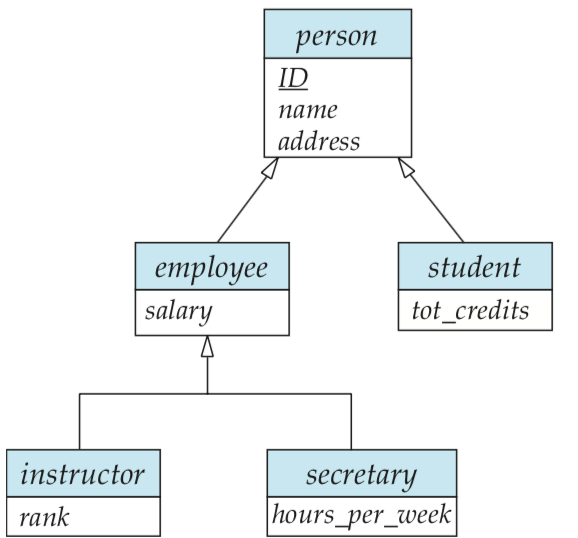
\includegraphics[width=0.35\textwidth]{images/specialization-generalization}\\
An E-R diagram showing specialization and generalization~\cite{dsc}.
\end{center}

We have some choices about how the generalization is defined. The first option is to have it be \textit{condition} defined, such as having some rules that say that a person who fulfills a certain condition is included in that group. So a customer who has status of ``Frequent Flyer'' in the system is automatically included in that specialization. In other cases, an operation must be taken to specifically include a person in that subset, such as assigning an employee to a specific department~\cite{dsc}. 

We could also have rules that say sets must be disjoint (a member of some group cannot be a member of another group), or if they can be overlapping. In our system we could say that a staff person can also be a customer, but that is specific  to the domain we are discussing. 

We can also have the idea of an ``abstract class'': we could write in some rules that say that no instance of ``user'' can exist, and everyone must be a staff member or customer (or both). In that case, this is called total specialization: we are not allowed to have unspecialized (general) entities. The entity user might appear in the E-R diagram but as notational convenience only.

\paragraph{Aggregation.} 

Aggregation allows us to treat a grouping of entities that are related as a single block. This can simplify the diagram and show us a relationship between relationships. Aggregation may not seem very useful in the context of a database schema that can be handily represented on a piece of paper, but for a large database it can be a good way to sequester parts of the design in a different area so the diagram is comprehensible.

The scenario we'll do has to do with a four-way relationship between instructor, student, project, and evaluation. In this scenario, hopefully a realistic one, there is a student project that is supervised and evaluated by an instructor. The evaluation belongs to the relationship ``project guide'', which is defined by the three elements of (instructor, student, project). Actually, the name project guide is probably unclear. If it were up to me I would call the ``project'' relation ``topic'' and the ``proj\_guide'' relationship would be ``project''. 

\begin{center}
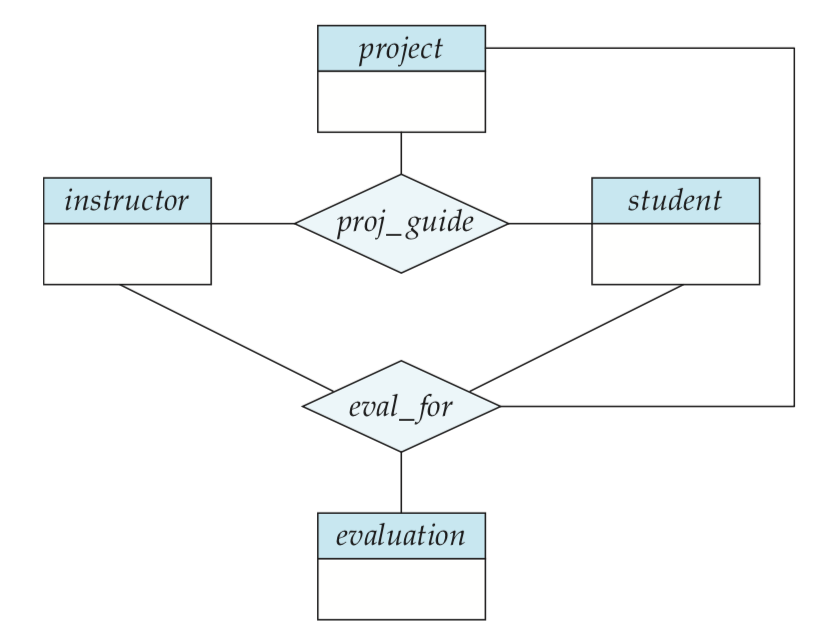
\includegraphics[width=0.45\textwidth]{images/unaggregated}
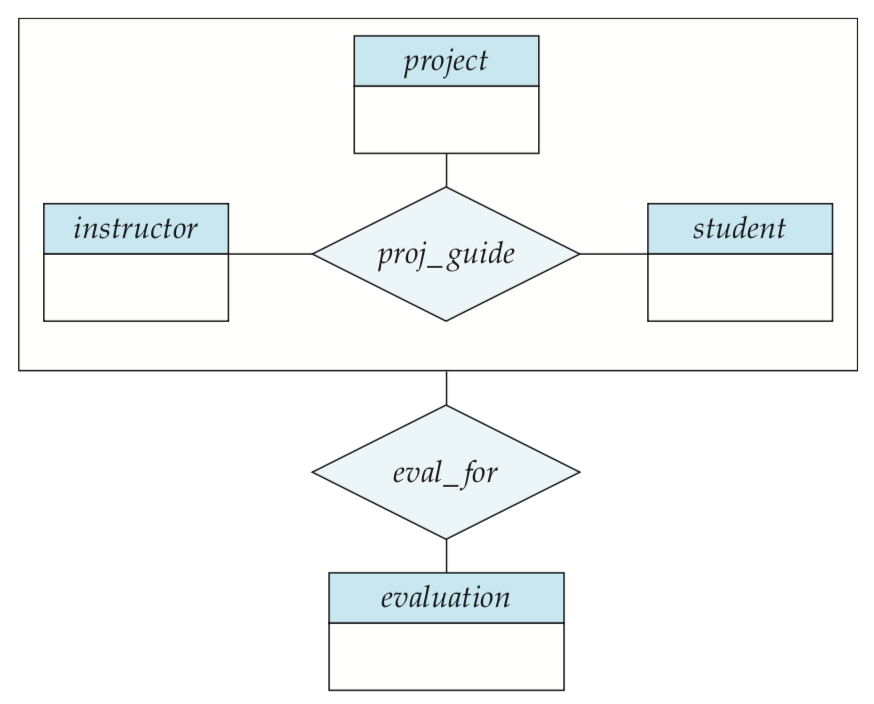
\includegraphics[width=0.42\textwidth]{images/aggregation}\\
E-R diagram with complex relationship without (left) and with (right) aggregation~\cite{dsc}.
\end{center}

It looks like the relationship \textit{eval\_for} and \textit{proj\_guide} can be combined because they seem to connect the same three things. But we may not want to do that if some sets of (instructor, student, project) do not have an associated evaluation. Now possibly the data is redundant; if the evaluation is a simple enough element (e.g., it is an enumeration or an integer letter grade) then it could be an attribute of the \textit{proj\_guide} relationship. But this option is not suitable if the evaluation relation is used in some other relationship or in some other context. We  also might not be able to combine it if there are multiple evaluations on a project...~\cite{dsc}.

Conceptually we might prefer to think of \textit{proj\_guide} as a higher level entity,  leaving a binary relationship between that aggregated entity and the evaluation relation.

It is worth noting that the textbook contains a couple of alternative diagram notations. You may encounter them in the real world, but we will not invest any time discussing them as they could be confusing.

Given a good understanding of how diagrams are formed, we will next think about how to turn models into tables, and what makes up a good design.

\bibliographystyle{alphaurl}
\bibliography{356}


\end{document}
